\section {PlanesWidget}

\subsection{MainWindow}

The GUI is hosted by a QMainWindow of the derived class PlanesWWindow. The constructor of PlanesWWindow creates the game controller (a PlaneRound object) and gives it as parameter to the central area of the QMainWindow, which is an object of the class PlanesWView.


\begin{lstlisting}
PlanesWWindow::PlanesWWindow(QWidget *parent) :
	QMainWindow(parent)
{
	//builds the game object - the controller
	mRound = new PlaneRound(10, 10, 3);
	
	//builds the view object
	mPlanesView = new PlanesWView(mRound);
	setCentralWidget(mPlanesView);
	
	//starts the game
	mRound->initRound();
}

\end{lstlisting}

PlanesWView creates in the constructor the layout of the GUI. In Figure \ref{fig:planeswidget_game_widgetnames} are shown the names of the widgets used in the game area layout.

\begin{figure}[h]
	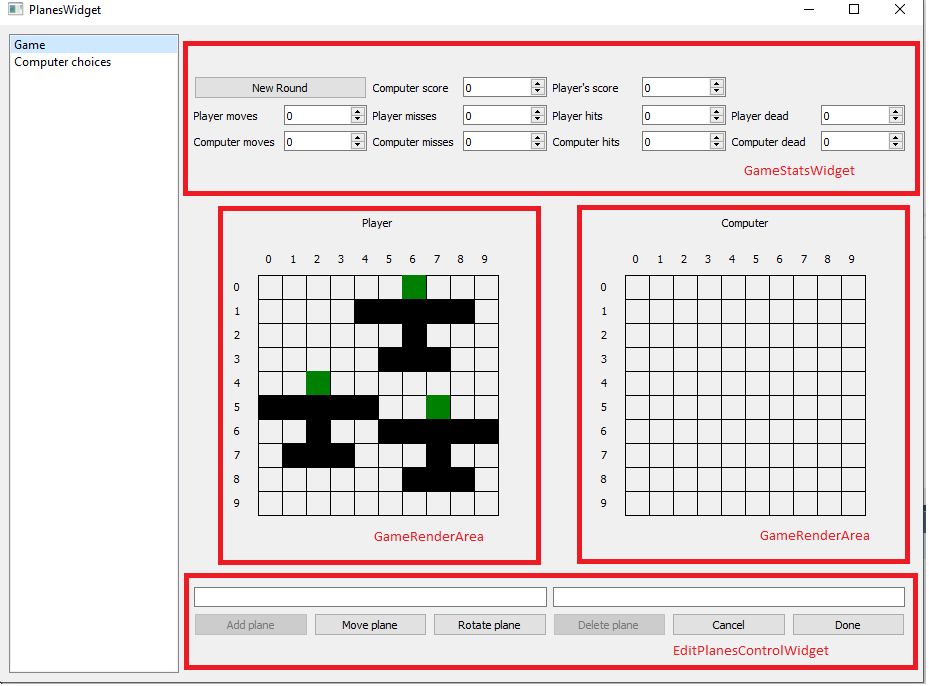
\includegraphics[width = \textwidth]{PlanesWidget_Game_WidgetNames.png}
	\caption{Widgets in the game area layout}
	\label{fig:planeswidget_game_widgetnames}
\end{figure}

\subsection {Qt Concepts}

\subsubsection {QMainWindow}
\subsubsection {QWidget}